\section{What is aging?}

\subsection{Definition and Hallmarks}

\begin{frame}[c]{Aging}
    \large
    
    \begin{block}{Definition}
        Ageing is characterized by a progressive decline in organismal fitness
        occurs with increasing age, ultimately ending in death.  CITE!!
    \end{block}
    \pause
    But how can we measure it?
\end{frame}


\begin{frame}[c]{Hallmarks of Aging}
    According to \cite{lopez2013hallmarks}:
    \begin{itemize}[<+(1)->]
        \item Genomic instability
        \item Telomere attrition
        \item Epigenetic alterations
        \item Loss of proteostasis
        \item Deregulated nutrient-sensing
        \item Mitochondrial dysfunction
        \item Cellular senescence
        \item Stem cell exhaustion
        \item Altered intercellular communication
    \end{itemize}
    \pause
    Hallmarks are mostly just side-effects we can measure!
\end{frame}


\subsection{Common Root Cause Existence}

\begin{frame}[c]{Life Expectancy after Cancer}
    \large
    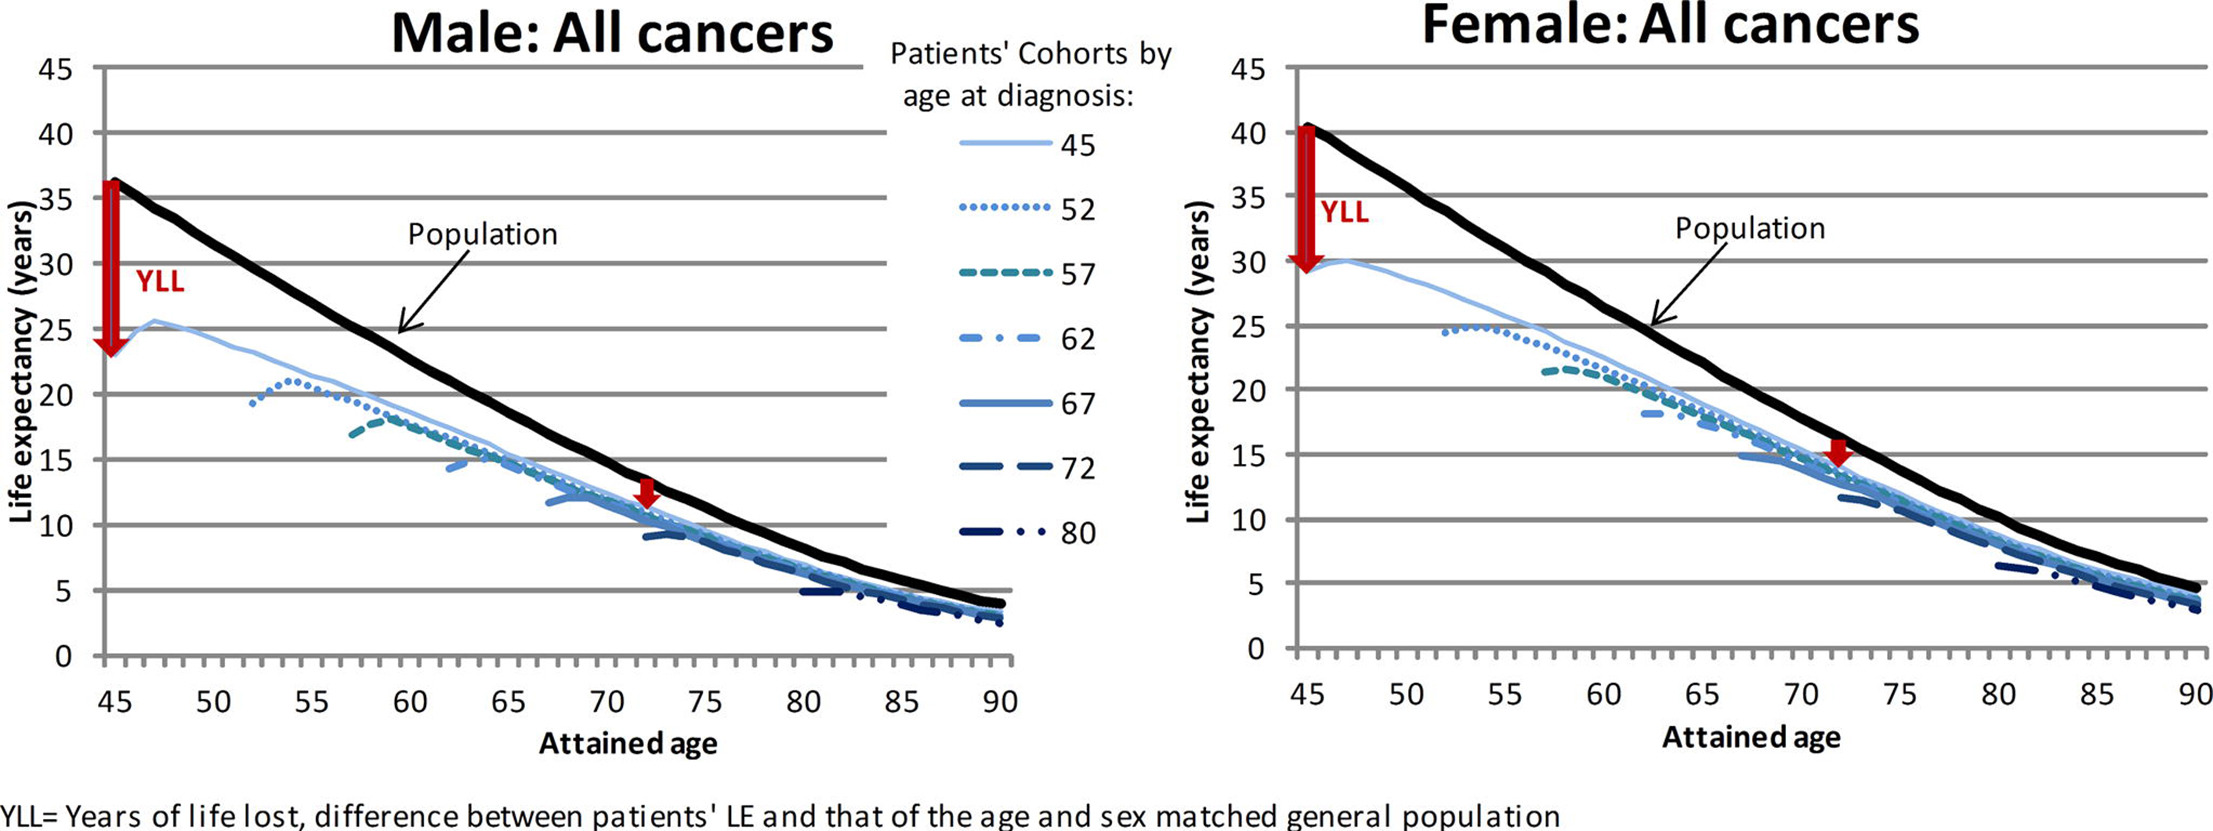
\includegraphics[width=\textwidth]{all_cancers_LE} \\
    \cite{botta2019changes}
    \newline
    \newline
    \pause
    Conclusion: Cancer causes the underlying \\ 'aging clock' to speed up
\end{frame}

\begin{frame}[c]{Life Expectancy with Diabetes}
    \large
    Life Expectancy is at least 10 years lower with Diabetes Type 1
    \cite{livingstone2015estimated} and at least 5 years lower with Diabetes Type
    2 \cite{untitled1:online}.
    \newline
    \newline
    \pause
    Conclusion: Diabetes causes the underlying \\ 'aging clock' to speed up
\end{frame}


\begin{frame}[c]{Similarity of diseases of aging}
    \large
    \cite{CorePath13:online}
    At the cellular level:
    \begin{itemize}[<+(1)->]
        \item decrease in cell count
        \item increase in damaged proteins/DNA/fats
        \item inflammation
    \end{itemize}
    \pause

    Roughly this pattern for:
    \begin{itemize}[<+(1)->]
        \item alzheimers
        \item atherosclerosis
        \item muscle loss
        \item many others
    \end{itemize}
\end{frame}


\begin{frame}[c]{Existence proof for common pathways}
    \large
    \begin{aquote}{John S Wentworth}
        someone who has one severe illness early is likely to have others
    \end{aquote}

    \pause
    Most severe illnesses cause the 'aging clock' to speed up. Most diseases of
    aging have similar characteristics. This is direct evidence that there are
    {\em few underlying root causes} for aging.
\end{frame}




\subsection{Assumed Root Causes}


\begin{frame}[c]{Mitochondrial dysfunction}
    \large
    Turns out, mitochondrial dysfunction accounts for telomere-dependent senescence \cite{passos2007mitochondrial}.
\end{frame}


\begin{frame}[c]
    \large
    Assumed root causes: free radicals and transposon damage \\
    Maybe not in too much detail? Could fill 30min itself \cite{CorePath13:online} \\
    \pause

    p21 and reactive oxygen feedback for senescence \cite{passos2010feedback}
\end{frame}

